% !TEX program = lualatex
\documentclass[border=6pt]{standalone}
% ---------------------------------------------------------------------------
% tikzpreamble.tex -- shared by main.tex and by every standalone in tikz/
% ---------------------------------------------------------------------------
\usepackage{amsmath}
\usepackage{amssymb}
\usepackage{tikz}
\usepackage{circuitikz}
\usetikzlibrary{arrows.meta,calc,positioning,decorations.pathmorphing,decorations.pathreplacing,
                decorations.markings,patterns,angles,quotes,fit,
                shapes.geometric,shapes.misc,backgrounds,intersections}

\ctikzset{bipoles/length=0.85cm}
\ctikzset{resistors/scale=0.85}
\ctikzset{capacitors/scale=0.9}

\tikzset{
  wire/.style      = {line width=0.7pt},
  dashedwire/.style= {line width=0.7pt, densely dashed},
  term/.style      = {circle, draw, line width=0.6pt, fill=white,
                      inner sep=0pt, minimum size=4.5pt},
  node dot/.style  = {circle, fill=black, inner sep=0pt, minimum size=4pt},
  boxlabel/.style  = {font=\sffamily\small},
  annot/.style     = {font=\small, align=left},
  phasor/.style    = {-{Stealth[length=3.2mm,width=2.2mm]}, line width=1.1pt},
  thinphasor/.style= {-{Stealth[length=2.6mm,width=1.8mm]}, line width=0.7pt},
  axis line/.style = {-{Stealth[length=2.6mm,width=1.8mm]}, line width=0.6pt},
  guide/.style     = {densely dashed, line width=0.4pt, gray},
}
\usepackage{siunitx}

\begin{document}
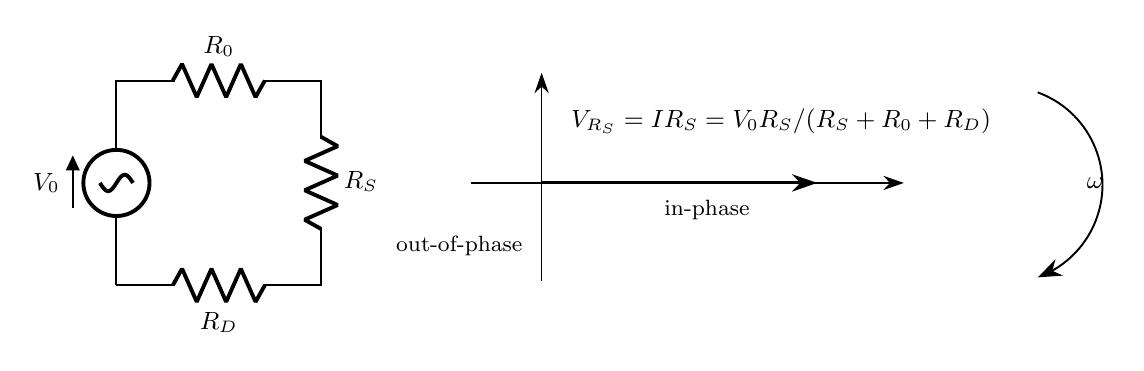
\begin{tikzpicture}[every node/.style={font=\small}]

  % ---- circuit -----------------------------------------------------------
  \begin{scope}[shift={(0,0)}]
    \draw[wire] (0,0) to[sV=$V_0$,invert] (0,2.6)
                      to[R=$R_0$] (2.6,2.6)
                      to[R=$R_S$] (2.6,0)
                      to[R=$R_D$] (0,0);
  \end{scope}

  % ---- phasor diagram ----------------------------------------------------
  \begin{scope}[shift={(5.4,1.3)}]
    \draw[axis line] (0,-1.25) -- (0,1.4);
    \draw[axis line] (-0.9,0)  -- (4.6,0);
    \node[anchor=north east,font=\footnotesize] at (-0.12,-0.55) {out-of-phase};
    \node[anchor=north,font=\footnotesize] at (2.1,-0.1) {in-phase};
    \draw[phasor] (0,0) -- (3.5,0);
    \node[anchor=south west] at (0.25,0.5)
      {$V_{R_S}=I R_S = V_0 R_S/(R_S+R_0+R_D)$};
    % rotation arrow
    \draw[-{Stealth[length=3mm]},line width=0.7pt]
      (6.3,1.15) arc[start angle=70,end angle=-70,radius=1.25];
    \node[anchor=west] at (6.8,0) {$\omega$};
  \end{scope}
\end{tikzpicture}
\end{document}
